\documentclass{beamer}
%\documentclass[handout]{beamer} %use this for no pauses or backup slides

\mode<presentation>
{
  \definecolor{berkeleyblue}{HTML}{003262}
  \definecolor{berkeleygold}{HTML}{FDB515}
  \usetheme{Boadilla}      % or try Darmstadt, Madrid, Warsaw, ...
  %\usecolortheme{dove} % or try albatross, beaver, crane, ...
  \setbeamercolor{structure}{fg=berkeleyblue,bg=berkeleygold}
  \setbeamercolor{palette primary}{fg=berkeleyblue,bg=berkeleygold} % changed this
  \setbeamercolor{palette secondary}{bg=berkeleyblue,fg=white} % changed this
  \setbeamercolor{palette tertiary}{fg=berkeleyblue,bg=berkeleygold} % changed this
  \usefonttheme{structurebold}  % or try serif, structurebold, ...
  \useinnertheme{circles}
  \setbeamertemplate{navigation symbols}{}
  \setbeamertemplate{caption}[numbered]
  \usebackgroundtemplate{}
}

\setbeamertemplate{footline}
{
  \leavevmode%
  \hbox{%
  \begin{beamercolorbox}[wd=0.25\paperwidth,ht=2.25ex,dp=1ex,center]{author in head/foot}%
    \usebeamerfont{author in head/foot}\insertshortauthor
  \end{beamercolorbox}%
  \begin{beamercolorbox}[wd=0.75\paperwidth,ht=2.25ex,dp=1ex,center]{title in head/foot}%
    \usebeamerfont{title in head/foot}\insertshorttitle\hspace*{3em}
    \insertframenumber{} / \inserttotalframenumber\hspace*{1ex}
  \end{beamercolorbox}}%
  \vskip0pt%
}

\setbeamertemplate{frametitle continuation}{}
\newcounter{multipleslide}

\newcommand{\backupbegin}{
   \newcounter{framenumberappendix}
   \setcounter{framenumberappendix}{\value{framenumber}}
}
\newcommand{\backupend}{
   \addtocounter{framenumberappendix}{-\value{framenumber}}
   \addtocounter{framenumber}{\value{framenumberappendix}} 
}

\newcommand{\vars}{\raisebox{0pt}[1ex][1ex]{S}}

\usepackage{bmpsize}
\usepackage{tikz}
\usepackage{tikz-3dplot}
\usetikzlibrary{arrows}
\usetikzlibrary{decorations.pathreplacing}
\usetikzlibrary{3d,angles,quotes,calc}
\usepackage{environ}

\makeatletter%
\newcommand{\multipleframe}{%
\setcounter{multipleslide}{\value{framenumber}}
\stepcounter{multipleslide}
\patchcmd{\beamer@@tmpl@footline}% <cmd>
  {\insertframenumber}% <search>
  {\themultipleslide}% <replace>
  {}% <success>
  {}% <failure>
}
\newcommand{\restoreframe}{%
\patchcmd{\beamer@@tmpl@footline}% <cmd>
  {\themultipleslide}% <search>
  {\insertframenumber}% <replace>
  {}% <success>
  {}% <failure>
\setcounter{framenumber}{\value{multipleslide}}%
}
\newsavebox{\measure@tikzpicture}
\NewEnviron{scaletikzpicturetowidth}[1]{%
  \def\tikz@width{#1}%
  \def\tikzscale{1}\begin{lrbox}{\measure@tikzpicture}%
  \BODY
  \end{lrbox}%
  \pgfmathparse{#1/\wd\measure@tikzpicture}%
  \edef\tikzscale{\pgfmathresult}%
  \BODY
}
\makeatother%

\newenvironment{cframed}[1][black]
  {\def\FrameCommand{\fboxsep=\FrameSep\fcolorbox{#1}{white}}%
    \MakeFramed {\advance\hsize-\width \FrameRestore}}
  {\endMakeFramed}

\newcommand\scalemath[2]{\scalebox{#1}{\mbox{\ensuremath{\displaystyle #2}}}}

\usepackage{amssymb}
\usepackage{amsmath}
\usepackage[sorting=none,backend=biber]{biblatex}
\usepackage{fancyvrb}
\usepackage{caption}
\usepackage[version=3]{mhchem}
\usepackage{etoolbox}
\usepackage{framed}
\usepackage[caption=false]{subfig}
\usepackage{stmaryrd} % for short right arrow
\usepackage{multirow}
\usepackage[super]{nth}
\usepackage{color, colortbl}
\usepackage{hyperref}

\definecolor{LightRed}{rgb}{1,.8,.8}

\newcommand{\bo}{\mathbf\Omega}
\newcommand{\vecr}{\textbf{r}}
\newcommand{\sn}{S$_\mathrm{N}$}
\newcommand{\pn}{P$_\mathrm{N}$}
\newcommand{\sigt}{\Sigma_t}
\newcommand{\sigs}{\Sigma_s}
\newcommand{\sa}{\shortrightarrow}
\newcommand{\Ye}[2]{\ensuremath{Y^e_{#1}(\bo_#2)}}
\newcommand{\Yo}[2]{\ensuremath{Y^o_{#1}(\bo_#2)}}
\newcommand{\E}[1]{$\times10^{#1}$}
\newcommand{\mr}[1]{\multirow{2}{*}{#1}}
\newcommand{\ve}[1]{\ensuremath{\mathbf{#1}}}
\newcommand{\psid}{\psi^{\dagger}}
\newcommand{\cpp}{C\nolinebreak\hspace{-.05em}\raisebox{.4ex}{\tiny\bf +}\nolinebreak\hspace{-.10em}\raisebox{.4ex}{\tiny\bf +}}

\bibliography{2019-siam-cse}
\setbeamertemplate{bibliography item}[text]
\renewcommand*{\bibfont}{\scriptsize}

\title[Assessment of the LDO Equations for 3D Neutral Particle Transport]
{Assessment of the Lagrange Discrete Ordinates Equations for Three-dimensional Neutral Particle Transport}
\author[Kelly L. Rowland et al.]{Kelly L. Rowland, Cory D. Ahrens, Steven Hamilton, Rachel N. Slaybaugh}
% \institute{Department of Nuclear Engineering\\University of California, Berkeley}
\date{SIAM CSE 2019}
\begin{document}

\begin{frame}[plain]
	\titlepage
\end{frame}

\begin{frame}{Radiation Transport}
%
\pause
%
\center
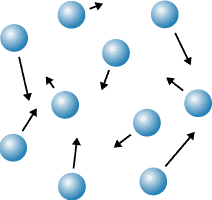
\includegraphics[width=0.25\textwidth,natwidth=212,natheight=200]{img/particles.png}
%
\pause
%
\begin{columns}
\begin{column}{0.5\textwidth}
\center
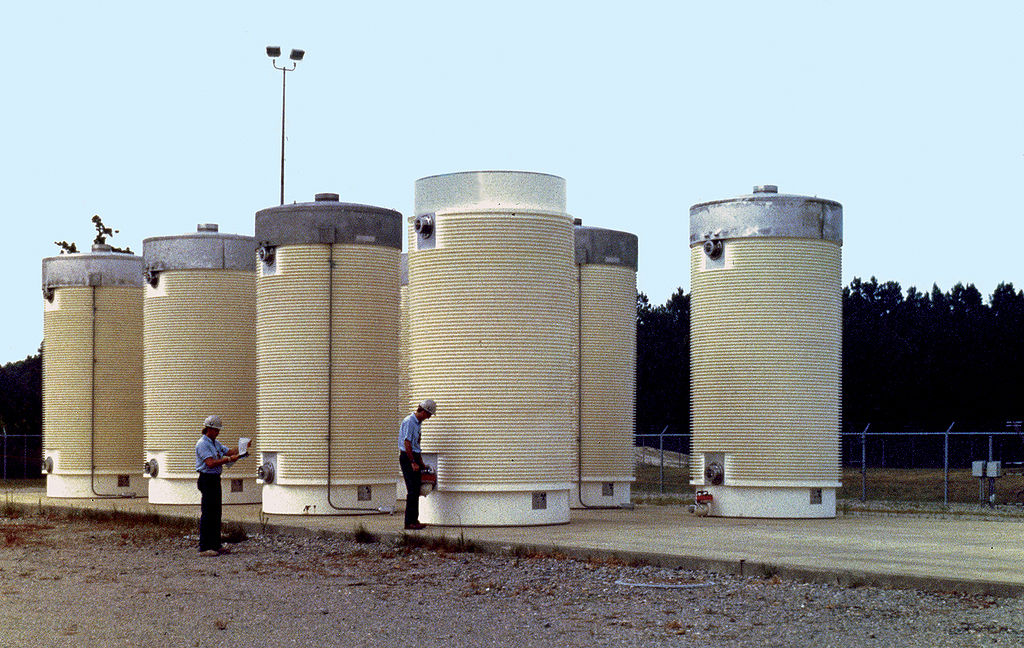
\includegraphics[width=\textwidth,natwidth=1024,natheight=648]{img/nuclear_dry_storage.jpg}
\end{column}
\begin{column}{0.5\textwidth}
\center
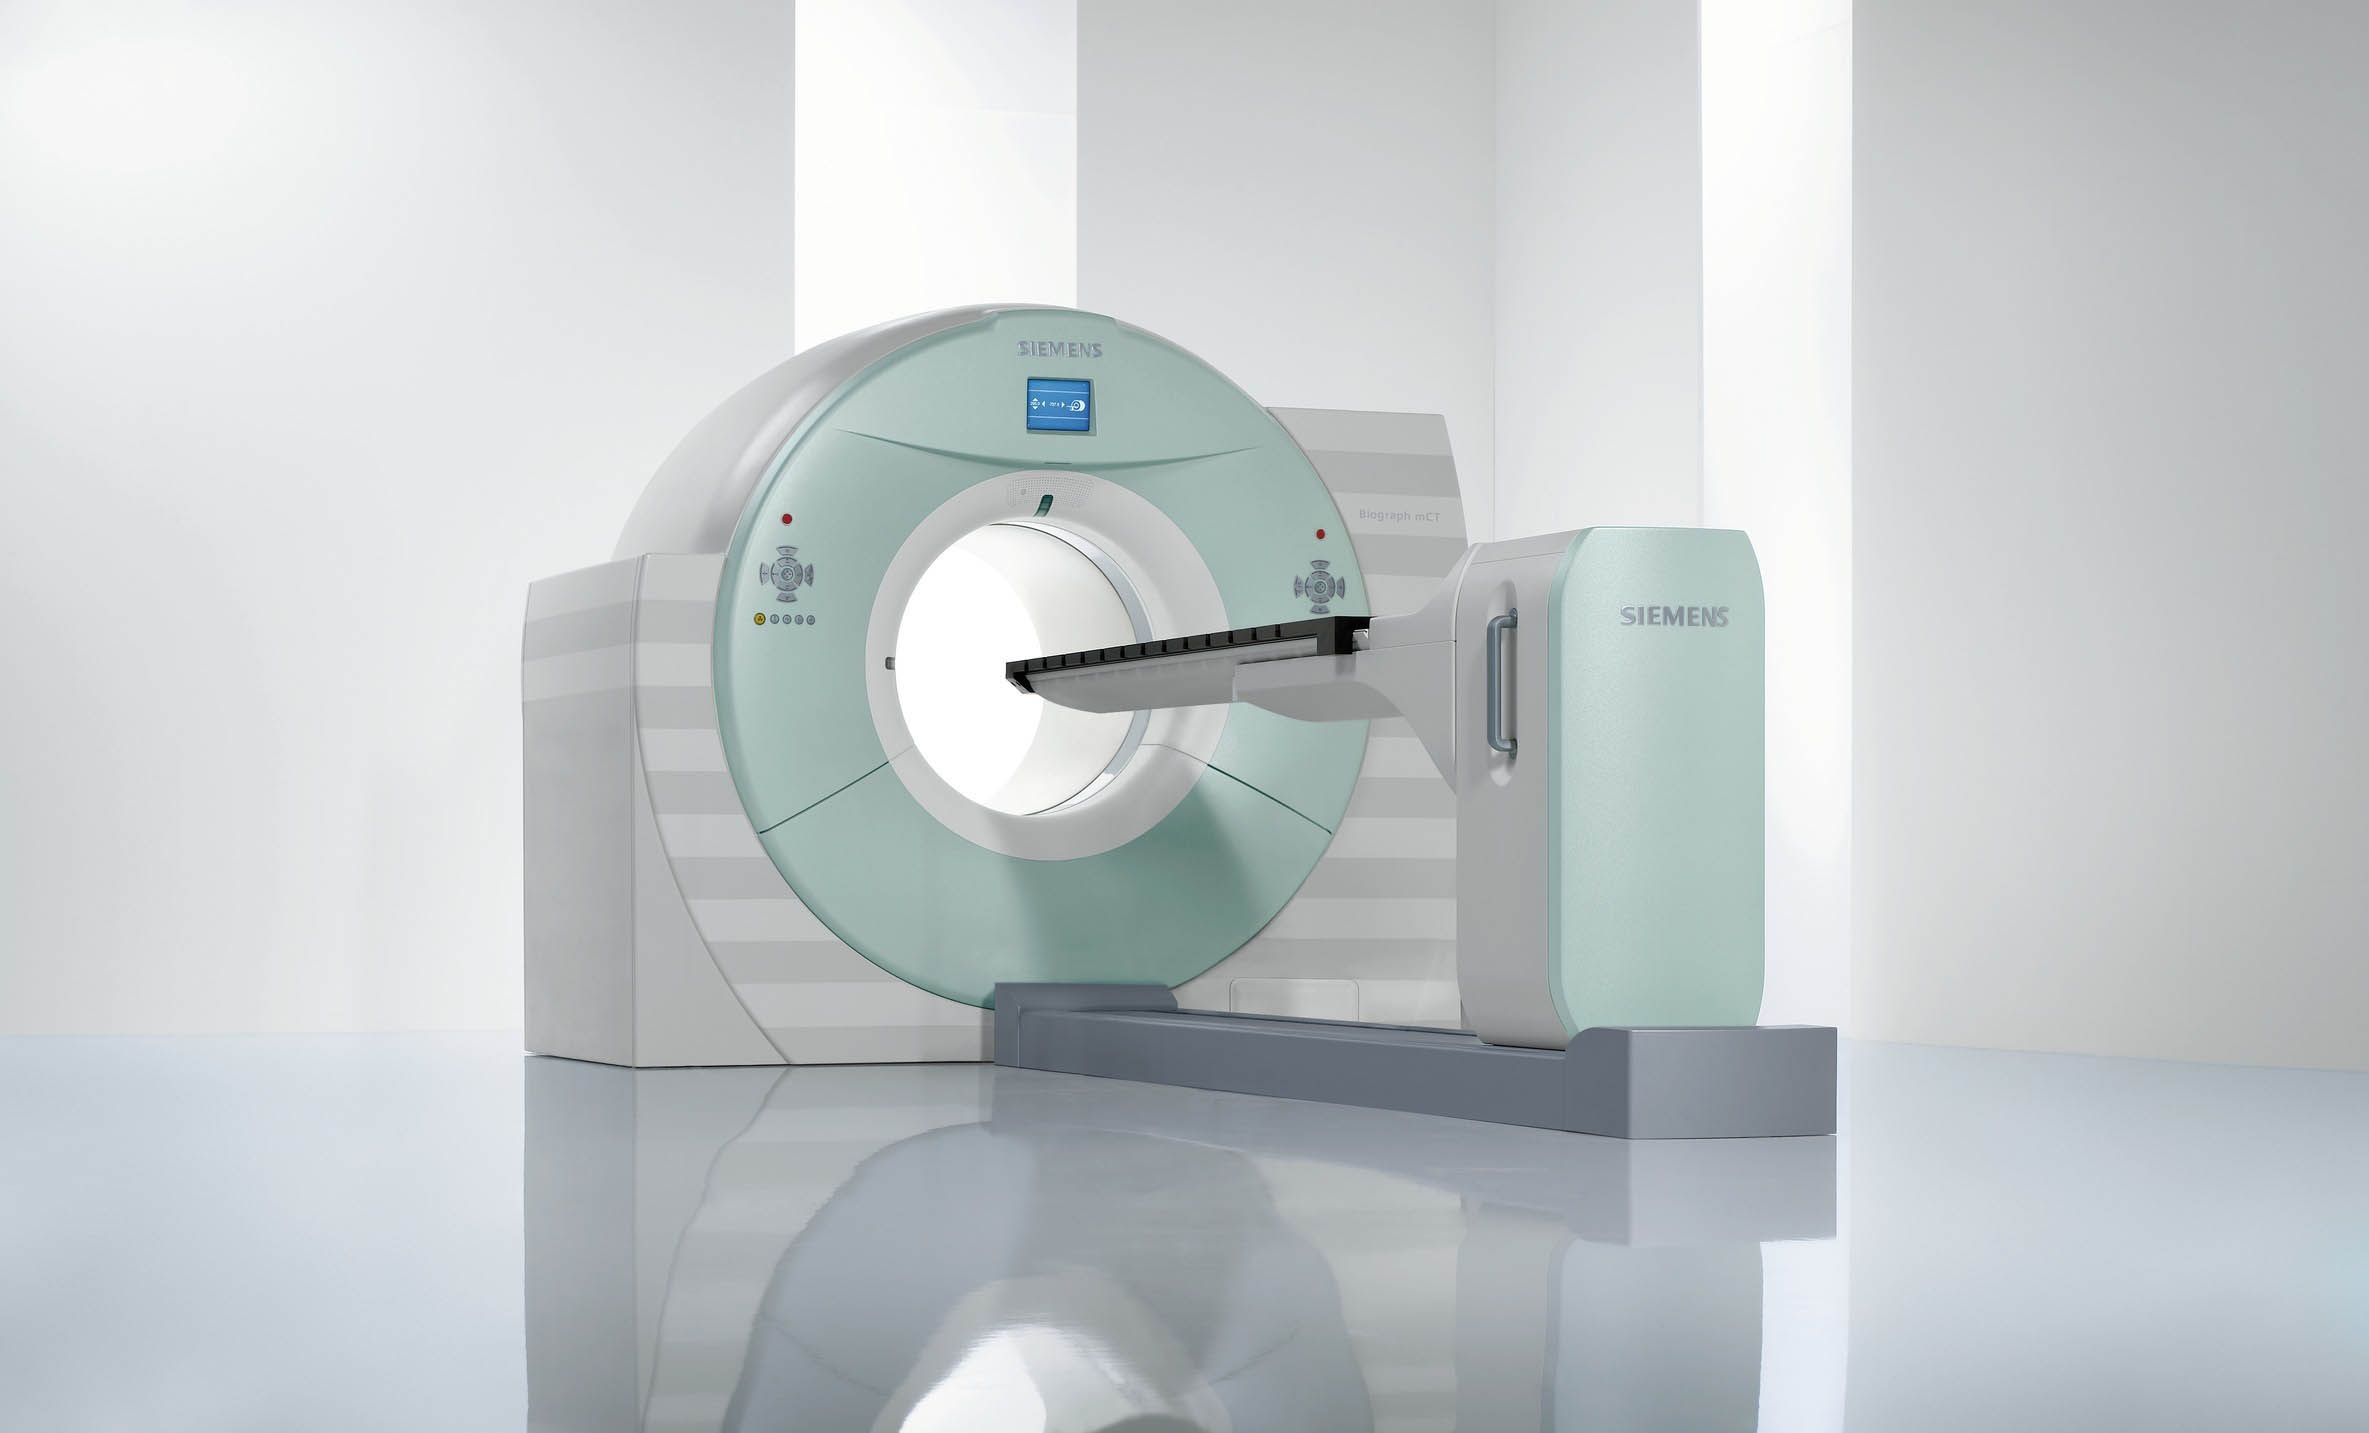
\includegraphics[width=\textwidth,natwidth=2369,natheight=1433]{img/pet-spect.jpg}
\end{column}
\end{columns}
%
\end{frame}

\begin{frame}{Numerical Methods for Radiation Transport}
%
\begin{columns}
\begin{column}{0.5\textwidth}
\begin{itemize}
\item{We need predictive simulation}
\item{Translate applied math into code used to design and analyze nuclear systems}
\item{Use high performance computing}
\item{Inform algorithm development with physics of problems of interest}
\end{itemize}
\end{column}
\begin{column}{0.5\textwidth}
\center

\includegraphics[width=0.7\textwidth,natwidth=465,natheight=340]{img/applied-math.jpg}

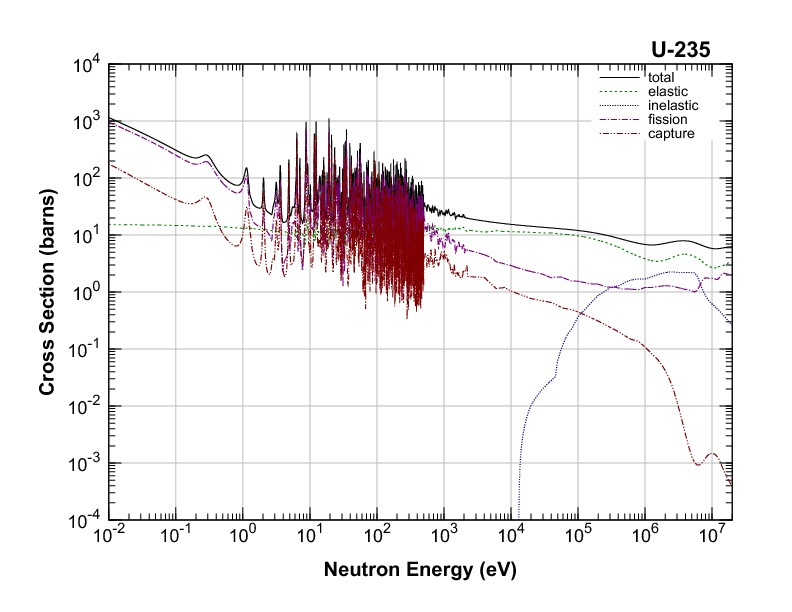
\includegraphics[width=\textwidth,natwidth=792,natheight=612]{img/u235-xsecs.jpg}
\end{column}
\end{columns}
%
\end{frame}

\begin{frame}{Outline}
  \begin{itemize}
  \item{Background}
  \item{Problem}
  \item{Results}
  \item{Summary}
  \end{itemize}
\end{frame}

\begin{frame}{Solving the Transport Equation}
%
\begin{multline*}
\bo \cdot \nabla \psi(\vecr,E,\bo) + \Sigma_t(\vecr,E) \psi(\vecr,E,\bo) = \\
\int_0^\infty\int_{4\pi} \Sigma_s(\vecr,E'\rightarrow E,\bo'\rightarrow\bo)
\psi(\vecr,E',\bo')d\bo'dE' + Q(\vecr,E,\bo)
\end{multline*}
%
\pause
%
\center
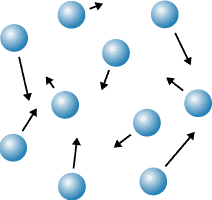
\includegraphics[width=0.25\textwidth,natwidth=212,natheight=200]{img/particles.png}
%
%
\end{frame}

\begin{frame}{Deterministic Solution Methods}
%
Discretize energy and space:
%%
\begin{columns}
\begin{column}{0.7\textwidth}
\begin{center}
\begin{scaletikzpicturetowidth}{0.8\textwidth}
\begin{tikzpicture}[scale=\tikzscale]
\draw[thick] (-5,0) -- (-3,0);
\draw[thick,dotted] (-3,0) -- (-1.5,0);
\draw[thick] (-1.5,0) -- (1.5,0);
\draw[thick,dotted] (1.5,0) -- (3,0);
\draw[thick,->] (3,0) -- (5.5,0);
\draw[thick] (-4.5,-0.25)--(-4.5,0.25);
\node [below] at (-4.5,-0.25) {\footnotesize$E_G$};
\draw[thick] (-3.5,-0.25)--(-3.5,0.25);
\node [below] at (-3.5,-0.25) {\footnotesize$E_{G-1}$};
\draw[thick] (-1,-0.25)--(-1,0.25);
\node [below] at (-1,-0.25) {\footnotesize$E_{g+1}$};
\draw[thick] (0,-0.25)--(0,0.25);
\node [below] at (0,-0.25) {\footnotesize$E_{g}$};
\node[above] at (-0.5, 0.25) {\footnotesize{group $g$}};
\draw[decorate,decoration={brace}](-1,0.275) -- (0,0.275);
\draw[thick] (1,-0.25)--(1,0.25);
\node [below] at (1,-0.25) {\footnotesize$E_{g-1}$};
\draw[thick] (3.5,-0.25)--(3.5,0.25);
\node [below] at (3.5,-0.25) {\footnotesize$E_1$};
\draw[thick] (4.5,-0.25)--(4.5,0.25);
\node [below] at (4.5,-0.25) {\footnotesize$E_0$};
\node [below] at (5.5,-0.1) {\footnotesize$E$};
\end{tikzpicture}
\end{scaletikzpicturetowidth}
\end{center}
%
\begin{center}
\begin{scaletikzpicturetowidth}{0.5\textwidth}
\begin{tikzpicture}[scale=\tikzscale]
\filldraw (xyz cs:x=-3,y=-3,z=3) circle (2pt) node {} -- 
          (xyz cs:x=3,y=-3,z=3) circle (2pt) node {};
\node[fill,circle,inner sep=0pt, minimum size = 2pt]%,
      % label={[shift={(-2.25,-0.75)}]
      % \footnotesize$(x_{i-1/2}, y_{j-1/2}, z_{k+1/2})$}] 
       at (xyz cs:x=-3,y=-3,z=3) {};
\node[fill,circle,inner sep=0pt, minimum size = 2pt]%,
      % label={[shift={(2,-0.75)}]
      % \footnotesize$(x_{i+1/2}, y_{j-1/2}, z_{k+1/2})$}] 
      at (xyz cs:x=3,y=-3,z=3) {};
\filldraw (xyz cs:x=-3,y=3,z=3) circle (2pt) node {} -- 
          (xyz cs:x=3,y=3,z=3) circle (2pt) node {};
 \node[fill,circle,inner sep=0pt, minimum size = 2pt]%,
%       label={[shift={(-2,-0.5)}]
%       \footnotesize$(x_{i-1/2}, y_{j+1/2}, z_{k+1/2})$}] 
       at (xyz cs:x=-3,y=3,z=3) {};
\node[fill,circle,inner sep=0pt, minimum size = 2pt]%,
      % label={[shift={(2,-0.5)}]
      % \footnotesize$(x_{i+1/2}, y_{j+1/2}, z_{k+1/2})$}] 
      at (xyz cs:x=3,y=3,z=3) {};
\filldraw (xyz cs:x=-3,y=3,z=3) -- 
          (xyz cs:x=-3,y=3,z=-3) circle (2pt) node[] {};
\node[fill,circle,inner sep=0pt, minimum size = 2pt]%,
      % label={[shift={(-2.25,-0.50)}]
      % \footnotesize$(x_{i-1/2}, y_{j+1/2}, z_{k-1/2})$}] 
      at (xyz cs:x=-3,y=3,z=-3) {};
\filldraw (xyz cs:x=3,y=3,z=3)  -- 
          (xyz cs:x=3,y=3,z=-3) circle (2pt) node {};
\node[fill,circle,inner sep=0pt, minimum size = 2pt]%,
      % label={[shift={(1.75,-0.50)}]
      % \footnotesize$(x_{i+1/2}, y_{j+1/2}, z_{k-1/2})$}] 
      at (xyz cs:x=3,y=3,z=-3) {};
\filldraw (xyz cs:x=3,y=-3,z=3) -- 
          (xyz cs:x=3,y=-3,z=-3) circle (2pt) node {};
\node[fill,circle,inner sep=0pt, minimum size = 2pt]%,
      % label={[shift={(1.75,-0.5)}]
      % \footnotesize$(x_{i+1/2}, y_{j-1/2}, z_{k-1/2})$}]
      at (xyz cs:x=3,y=-3,z=-3) {};
\draw (xyz cs:x=-3,y=-3,z=3) -- (xyz cs:x=-3,y=3,z=3);
\draw (xyz cs:x=3,y=-3,z=3) -- (xyz cs:x=3,y=3,z=3);
\draw (xyz cs:x=-3,y=3,z=-3) -- (xyz cs:x=3,y=3,z=-3);
\draw (xyz cs:x=3,y=-3,z=-3) -- (xyz cs:x=3,y=3,z=-3);
\node[fill,circle,inner sep=0pt, minimum size = 2pt]%,
      % label={[shift={(-2,-0.5)}]
      % \footnotesize$(x_{i-1/2}, y_{j-1/2}, z_{k-1/2})$}] 
      at (xyz cs:x=-3,y=-3,z=-3) {};
\filldraw[dashed] (xyz cs:x=-3,y=-3,z=-3) circle (2pt) node {} -- 
                  (xyz cs:x=-3,y=3,z=-3);
\draw[dashed] (xyz cs:x=-3,y=-3,z=-3) -- (xyz cs:x=3,y=-3,z=-3);
\draw[dashed] (xyz cs:x=-3,y=-3,z=-3) -- (xyz cs:x=-3,y=-3,z=3);
\filldraw (xyz cs: x=0,y=0,z=0) circle (2pt) node[below] 
          {\footnotesize$(x_i, y_j, z_k)$};
\end{tikzpicture}
\end{scaletikzpicturetowidth}
\end{center}
\end{column}
%
\begin{column}{0.3\textwidth}
\begin{align*}
\begin{split}
g &= 0,1,\ldots,G-1,\\
i &= 1,2,\ldots,I,\\
j &= 1,2,\ldots,J,\\
k &= 1,2,\ldots,K.
\end{split}
\end{align*}
\end{column}
\end{columns}
%
\pause
\centering
\vspace{1em}
\textcolor{red}{What about discretizing angle?}
%
\end{frame}

\begin{frame}{Discrete Ordinates Approximation}
%
\vspace{-2em}
%
\begin{multline*}
\bo_n \cdot \nabla \psi_n^g(\vecr) + \Sigma_t^g(\vecr)\psi_n^g(\vecr) = \\
\sum_{g'=0}^{G-1}\sum_{\ell=0}^{P}\Sigma_{s,\ell}^{g'\sa g}(\vecr)
\bigg[\Ye{\ell 0}{n}\phi_{\ell 0}^{g'}(\vecr) + \sum_{m=1}^{\ell}
\bigg(\Ye{\ell m}{n}\phi_{\ell m}^{g'}(\vecr) \\
 + \Yo{\ell m}{n}\vartheta_{\ell m}^{g'}(\vecr)\bigg)\bigg]
+ Q_n^g(\vecr)
\end{multline*}
%
\pause
%
\begin{columns}
\begin{column}{0.4\textwidth}

\includegraphics[width=\textwidth,natwidth=654,natheight=593]{img/ray-effects.png}
\end{column}
\pause
\begin{column}{0.2\textwidth}
\center\large increasing $N$
\vspace{-1.5em}
\center\Huge$\rightarrow$
\end{column}
\begin{column}{0.4\textwidth}

\includegraphics[width=\textwidth,natwidth=599,natheight=588]{img/ray-effects-fine.png}
\end{column}
\end{columns}
%
\end{frame}

\begin{frame}{Lagrange Discrete Ordinates (LDO) Equations \nocite{ahrens}}
%
\vspace{-2em}
% use energy group notation to be consistent with discrete ordinates eqs.
\begin{align*}
\bo_n\cdot\nabla\psi_{n}^g(\vecr) + 
&\Sigma_{t}^g(\vecr)\psi_{n}^g(\vecr) = \\
&\sum_{g'=0}^{G-1}\sum_{m=1}^{N}\sum_{n'=1}^{N}\langle L_{n'},L_{m}\rangle
\Sigma_{s,L}^{g'\sa g}(\vecr,\bo_{m}\cdot\bo_n)\psi_{n'}^{g'}(\vecr)
+ Q_{n}^g(\vecr)
\end{align*}
%
\pause
%
\begin{columns}
\begin{column}{0.4\textwidth}
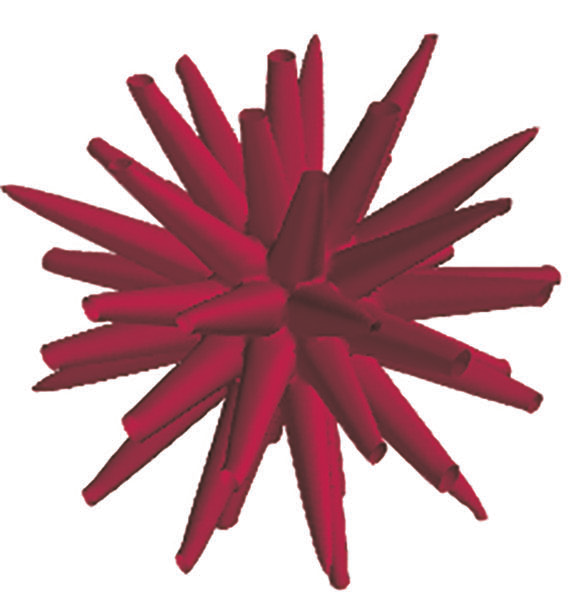
\includegraphics[width=\textwidth,natwidth=573,natheight=601]{img/ray-effects-ldo.png}
\end{column}
\pause
\begin{column}{0.2\textwidth}
\center\large increasing $N$
\vspace{-1.5em}
\center\Huge$\rightarrow$
\end{column}
\begin{column}{0.4\textwidth}

\includegraphics[width=\textwidth,natwidth=568,natheight=589]{img/ray-effects-fine-ldo.png}
\end{column}
\end{columns}
%
\end{frame}

\begin{frame}{Research Question}
%
\underline{Idea}: Implement the LDO equations in a radiation transport framework and
evaluate their solutions relative to standard quadrature sets.
%
\end{frame}

\begin{frame}{Software\nocite{denovo}}
%
\begin{columns}
\begin{column}{0.5\textwidth}
\begin{itemize}
\item{Exnihilo}
\begin{itemize}
\item{Framework including Denovo deterministic transport solver}
\item{Developed at Oak Ridge National Laboratory}
\item{\cpp, Python}
\end{itemize}
\end{itemize}
\end{column}
%
\begin{column}{0.5\textwidth}

\includegraphics[width=\textwidth,natwidth=932,natheight=754]{img/exnihilo.png}
\end{column}
\end{columns}
%
\end{frame}

\begin{frame}{Dog-Legged Void Neutron (DLVN) Benchmark}
%
\begin{columns}
\begin{column}{0.5\textwidth}
\begin{itemize}
\item{Designed to measure neutron streaming in iron with air voids}
\item{Iron and polyethylene}
\item{$40\times54\times48$ inches}
\item{Cf-252 point source located at center of $x-$ and $y-$directions at $z = 9$ inches}
\item{Symmetric about $y-z$ plane at $x = 0$}
\item{Modeled with vacuum boundary conditions}
\item{\textbf{Difficult to solve accurately and quickly}}
\end{itemize}
\end{column}
%
\begin{column}{0.5\textwidth}
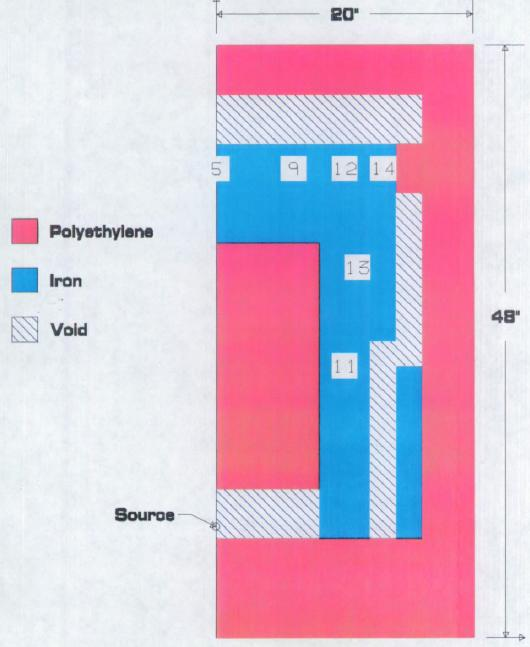
\includegraphics[width=\textwidth,natwidth=530,natheight=647]{img/dlvn.png}
\end{column}
\end{columns}

%
\end{frame}

\begin{frame}{DLVN Forward and Adjoint Solutions}
%
\begin{columns}
\begin{column}{0.45\textwidth}
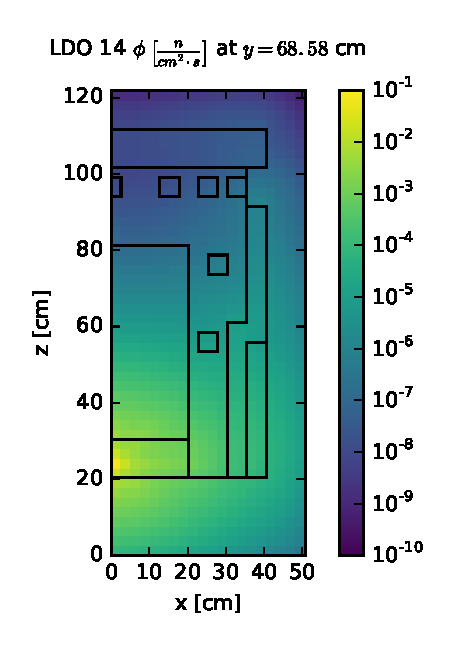
\includegraphics[width=\textwidth]{img/flux-ldo14-slice.eps}
\end{column}
%
\begin{column}{0.45\textwidth}
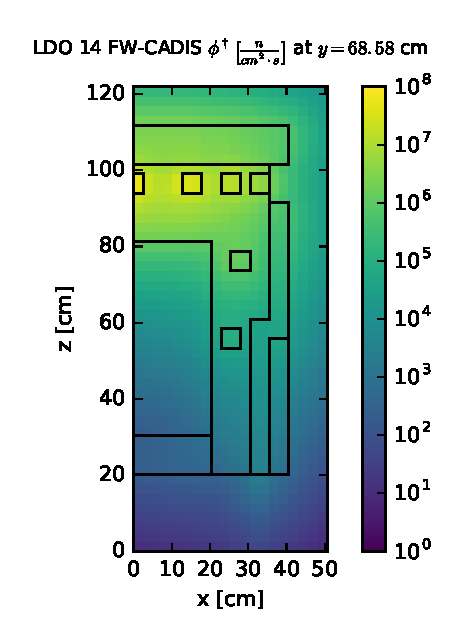
\includegraphics[width=\textwidth]{img/flux-ldo14-slice-adj.eps}
\end{column}
\end{columns}
%
\end{frame}

\begin{frame}{DLVN Benchmark Comparative Results}
Experimental and simulated scalar flux values [n/cm$^2$/s]:
\begin{table}[!htb]
% \centering
\scriptsize
\begin{tabular}{l|ccccccc}
              & Det. 5       & Det. 9    & Det. 11    & Det. 12
              & Det. 13      & Det. 14   \\ \hline
Exp.  & 6.97\E{-8}     & 1.57\E{-7}     & 8.81\E{-6}     & 2.60\E{-7}
              & 1.42\E{-6}     & 2.74\E{-7}     \rule{0pt}{2.6ex} \\
QR            & 4.98\E{-8}     & 1.68\E{-7}     & 8.65\E{-5}     & 4.92\E{-7}
              & 2.71\E{-6}     & 1.45\E{-6}     \\
Galerkin      & 3.24\E{-8}     & 1.47\E{-7}     & 8.19\E{-5}     & 4.43\E{-7}
              & 2.95\E{-6}     & 9.55\E{-7}     \\
LDFE          & 5.12\E{-8}     & 1.76\E{-7}     & 9.17\E{-5}     & 5.14\E{-7}
              & 2.93\E{-6}     & 1.47\E{-6}     \\
LDO           & 4.56\E{-8}     & 1.39\E{-7}     & 7.88\E{-5}     & 4.28\E{-7}
              & 2.37\E{-6}     & 1.28\E{-6}
\end{tabular}
\end{table}
%
Percent differences between experimental and simulated scalar flux values:
\begin{table}[!htb]
\small
\centering
\begin{tabular}{l|ccccccc}
              & Det. 5       & Det. 9    & Det. 11    & Det. 12
              & Det. 13      & Det. 14   \\ \hline
QR            & \textbf{25.58} & 6.89            & 881.94          & 89.09
              & 90.63          & 428.81          \\
Galerkin      & 53.48          & \textbf{6.37}   & 829.72          & 70.56
              & 107.7         & \textbf{248.42} \\
LDFE          & 26.61          & 12.3           & 940.41          & 97.75
              & 106.4         & 435.01          \\
\rowcolor{LightRed} LDO           & 34.61          & 11.2           & \textbf{794.75} & \textbf{64.46}
              & \textbf{66.77} & 368.24
\end{tabular}
\end{table}
\end{frame}

\begin{frame}{Summary}
%
\begin{itemize}
\item{Many radiation transport problems of interest are difficult to solve quickly with 
      high-quality answers}
\item{For problems with strong particle flux anisotropies, we need novel ways to incorporate
      angular information into solutions}
\item{LDO equations treat particle scattering differently than traditional discrete ordinates
      equations and incorporate angular information into scalar flux solutions in a new way}
\end{itemize}
%
\end{frame}

\begin{frame}{Acknowledgements}
\scriptsize
This material is based upon work supported under an Integrated
University Program Graduate Fellowship as well as supported by the Department 
of Energy under Award Number(s) DE-NE0008661. This report was prepared as an account 
of work sponsored by an agency of the United States Government. Neither the United 
States Government nor any agency thereof, nor any of their employees, makes any 
warranty, express or limited, or assumes any legal liability or responsibility for the 
accuracy, completeness, or usefulness of any information, apparatus, product, or
process disclosed, or represents that its use would not infringe privately owned
rights. Reference herein to any specific commercial product, process, or service by
trade name, trademark, manufacturer, or otherwise does not necessarily constitute or
imply its endorsement, recommendation, or favoring by the United States Government or
any agency thereof. The views and opinions of authors expressed herein do not 
necessarily state or reflect those of the United States Government or any agency 
thereof.
%
\centering

\includegraphics[width=\textwidth,natwidth=2539,natheight=1195]{img/DOE-IUP_Logo.png}
%
\end{frame}

\begin{frame}
  \huge{
  \begin{center}
  Questions?

  \vspace{\baselineskip}
  \url{https://tiny.cc/klr-nse18}
  \end{center}
  }
\end{frame}

\backupbegin
\begin{frame}[plain,allowframebreaks]{References}
\printbibliography
\end{frame}
\backupend

\end{document}